\documentclass[journal]{IEEEtran}

% -----------------------------------------------------------------------------
% Packages
% -----------------------------------------------------------------------------
\usepackage[utf8]{inputenc}
\usepackage[T1]{fontenc}
\usepackage{microtype}
\usepackage{amsmath,amssymb}
\usepackage{booktabs}
\usepackage{graphicx}
\usepackage{url}
\usepackage[hidelinks]{hyperref}
\usepackage[capitalise]{cleveref}
\crefname{figure}{Fig.}{Figs.}
\Crefname{figure}{Fig.}{Figs.}

\newcommand{\methodname}{Dueling Double DQN}
% Generated table rows are read with the primitive input: the robust \input of
% current LaTeX kernels breaks booktabs rules that follow it inside a tabular.
\makeatletter
\newcommand{\tablerows}[1]{\@@input #1 }
\makeatother

% -----------------------------------------------------------------------------
% Paper metadata
% -----------------------------------------------------------------------------
\title{Evaluating Cross-Level Generalization of a Dueling Double DQN
Trained in a Single Snake Environment}
\author{Nguyen~Duc~Manh and Hoang~Van~Anh%
\thanks{N. D. Manh and H. V. Anh are with FPT University (e-mail:
manhndse180326@fpt.edu.vn; anhhvse180142@fpt.edu.vn).}}

\begin{document}
\maketitle

% =============================================================================
% Abstract -- write this section last.
% =============================================================================
\begin{abstract}
Reinforcement-learning agents can achieve high scores in their training
environment while remaining sensitive to changes in environment geometry. This
study investigates whether a Dueling Double Deep Q-Network trained exclusively
on one level of the Snake game can transfer, without fine-tuning, to levels with
different board sizes and obstacle layouts. The agent is trained on a
$30\times30$ board and receives a fixed-dimensional 27-feature state vector with
three relative actions. We evaluate a frozen checkpoint greedily on the
training level and five unseen levels, using identical evaluation seeds and a
random-policy baseline. Performance is measured using score distributions,
target success rates, normalized scores, episode lengths, and termination
causes. Across 100 episodes per level, the selected checkpoint obtained an
in-domain mean score of $144.49\pm27.28$ on Level~4 and target success rates of
100\%, 97\%, 93\%, 74\%, and 54\% on Levels~1, 2, 3, 5, and 6, respectively;
the random baseline reached no target. Most failures on unseen levels were
early no-food timeouts while the snake was still short; episodes that reached
ten food items finished in 318 of 325 cases. For the evaluated policy, these results
show substantial zero-shot transfer, while the decline and high variance on the
two largest unseen levels show that cross-level generalization remains
incomplete. The study provides an empirical case study of both the opportunities
and limits of single-environment training in a parameterized Snake domain.
\end{abstract}

\begin{IEEEkeywords}
Reinforcement learning, Deep Q-Network, Double DQN, Dueling DQN,
generalization, zero-shot transfer, Snake.
\end{IEEEkeywords}

% =============================================================================
\section{Introduction}
\label{sec:introduction}

\IEEEPARstart{D}{eep} reinforcement learning (DRL) has produced agents that learn effective
control policies directly from interaction data. Deep Q-Networks (DQN), for
example, combine Q-learning \cite{watkins1992qlearning} with neural function
approximation, experience replay, and a target network
\cite{mnih2015human}. Later variants address specific weaknesses of the
original method: Double DQN reduces value overestimation
\cite{vanhasselt2016deep}, while the dueling architecture separately estimates
state value and action advantage \cite{wang2016dueling}. High performance in a
training environment, however, does not by itself demonstrate that the learned
policy will remain effective after the environment changes.

This distinction is especially important in game-based studies. An agent may
memorize regularities of one board size or obstacle arrangement rather than
learn a transferable navigation strategy. Generalization benchmarks in DRL
therefore separate the environments used for training from those used for
evaluation \cite{cobbe2020leveraging}. Snake offers a compact setting for this
question: board dimensions, obstacle layouts, and score targets can be changed
while the underlying transition rules and action semantics remain fixed. Prior
work has demonstrated that deep Q-learning can learn strong Snake policies and
has highlighted challenges caused by sparse rewards, moving targets, and the
increasing constraints produced by a growing body \cite{wei2018autonomous}.

We study a single-environment training setting. A \methodname{} agent is trained
only on Level~4, a $30\times30$ board with 20 static obstacle cells. The learned
network is then frozen and evaluated, without fine-tuning, on the training level
and five levels that were unseen during this training run. These levels range
from a $15\times15$ empty board to a $36\times36$ challenge board with 68
obstacle cells. A size-independent state representation and relative action
space allow the same network to operate on every board.

The study addresses the following research questions:

\begin{description}
  \item[RQ1] How well does a \methodname{} agent trained only on Level~4 perform
  on that same environment under greedy evaluation?
  \item[RQ2] To what extent does the frozen policy transfer, without
  fine-tuning, to Levels~1, 2, 3, 5, and 6?
  \item[RQ3] How do score, success rate, stability, and termination causes vary
  across levels with different board sizes and obstacle layouts?
\end{description}

This work makes the following contributions:

\begin{itemize}
  \item a parameterized Snake environment covering six board and obstacle
  configurations;
  \item a \methodname{} agent with a 27-feature, size-independent state encoding
  and three relative actions;
  \item a reproducible zero-shot evaluation protocol from one training level to
  five unseen levels; and
  \item an empirical analysis based on score distributions, target success,
  normalized performance, and failure modes.
\end{itemize}

The remainder of the paper reviews relevant work, describes the environment and
learning method, defines the experimental protocol, presents the results, and
discusses their implications and limitations.

% =============================================================================
\section{Related Work}
\label{sec:related-work}

\subsection{Value-Based Deep Reinforcement Learning}

Q-learning is an off-policy temporal-difference method that estimates the
optimal action-value function without requiring a model of the environment
\cite{watkins1992qlearning,sutton2018reinforcement}. For large state spaces, DQN
uses a neural network as the action-value approximator and stabilizes learning
with a replay buffer and a target network \cite{mnih2015human}. Standard DQN
uses the same maximization operation to select and evaluate the next action,
which can produce overestimated action values.
Double DQN separates these roles: the online network selects the maximizing
action, and the target network evaluates it \cite{vanhasselt2016deep}.

The dueling architecture decomposes the Q-value into a state-value term and an
action-advantage term \cite{wang2016dueling}. This design is useful when many
actions have similar effects in a given state. The present work combines Double
DQN targets with a dueling network and therefore refers to the agent as a
Dueling Double DQN.

\subsection{Generalization in Reinforcement Learning}

Generalization in RL concerns performance beyond the exact environments or
random seeds observed during training. CoinRun formalized distinct training and
test sets for RL and showed that agents can overfit even when trained on many
environment instances \cite{cobbe2019quantifying}. Procgen extended this line of
work with 16 procedurally generated environments and demonstrated the importance
of environment diversity for both training and evaluation
\cite{cobbe2020leveraging}. Kirk et al. survey zero-shot generalization in deep
RL and frame it with contextual Markov decision processes, in which training and
test environment instances differ \cite{kirk2023survey}. Our six levels form a
small, hand-designed instance of this setting. These studies motivate our strict
separation of the single source level from unseen evaluation levels.

Reliable generalization claims also require careful aggregation. Deep RL results
can vary substantially with random seeds, implementation details, and evaluation
choices \cite{henderson2018deep}. Point estimates alone can hide statistical
uncertainty, especially when only a few independently trained agents are
available \cite{agarwal2021deep}. Our paper therefore reports distributions and
quartiles and explicitly treats the single training seed as a limitation.

Unlike approaches that train on a distribution of environments, this study
deliberately uses only one training level. It asks whether a compact,
geometry-aware representation is sufficient for zero-shot transfer across
board sizes and obstacle layouts. The experiment therefore evaluates transfer
from a single source environment rather than the benefits of domain
randomization or curriculum learning.

\subsection{State Representations for Transfer}

A neural policy with raw board-sized input generally fixes the input geometry.
Our encoder instead maps every level to the same 27-dimensional feature vector.
Several features are normalized by board dimensions, while actions are defined
relative to the snake's current heading. This design makes cross-level execution
possible. Whether it produces effective transfer remains an empirical question;
the present experiment does not claim that representation invariance alone
guarantees behavioral generalization.

\subsection{Deep Reinforcement Learning for Snake}

Wei et al. applied a convolutional DQN variant to Snake and proposed reward,
training-gap, and dual-replay mechanisms for the game's sparse and changing
objectives \cite{wei2018autonomous}. Their work establishes Snake as a useful
DRL test bed, but focuses on improving performance within the game configuration
used for training. In contrast, the present study centers on a frozen policy's
cross-level behavior when board size and obstacle geometry change. This narrower
focus permits a direct distinction between in-domain performance and zero-shot
transfer, although our feature-vector representation is not directly comparable
to their stack of screen images.

% =============================================================================
\section{Methodology}
\label{sec:methodology}

\subsection{Parameterized Snake Environment}

At the beginning of each episode, a snake of length three is placed at a valid
random location facing right. Food is sampled uniformly from currently unoccupied
cells. Eating food increases the score by one and the snake length by one. An
episode terminates when the snake hits a wall, a static obstacle, or itself;
when no free cell remains; when it exceeds the no-food timeout; or, for levels
with a finite target, when it reaches that target.

The no-food timeout is twice the number of cells on the board. The counter is
reset whenever food is consumed. This termination rule prevents non-progressing
cycles without imposing a fixed total episode length. A timeout is a truncation
rather than a true terminal state. Following Pardo et al.
\cite{pardo2018time}, the released trainer stores timeout transitions as
non-terminal and keeps bootstrapping from the next state. In the
reported training run, no episode ended by timeout: all 19,094 completed
episodes ended in self, obstacle, or wall collision. This distinction therefore
did not affect the trained model.

\begin{table*}[t]
  \centering
  \caption{Environment configurations and their roles in the present study.}
  \label{tab:levels}
  \begin{tabular}{llrrrr}
    \toprule
    Level & Role & Height & Width & Obstacles & Target \\
    \midrule
    1 & Unseen evaluation & 15 & 15 & 0  & 25 \\
    2 & Unseen evaluation & 20 & 20 & 8  & 35 \\
    3 & Unseen evaluation & 24 & 24 & 16 & 50 \\
    4 & Training and in-domain evaluation & 30 & 30 & 20 & None \\
    5 & Held-out evaluation & 32 & 32 & 34 & 100 \\
    6 & Challenge evaluation & 36 & 36 & 68 & 150 \\
    \bottomrule
  \end{tabular}
\end{table*}

\begin{figure*}[t]
  \centering
  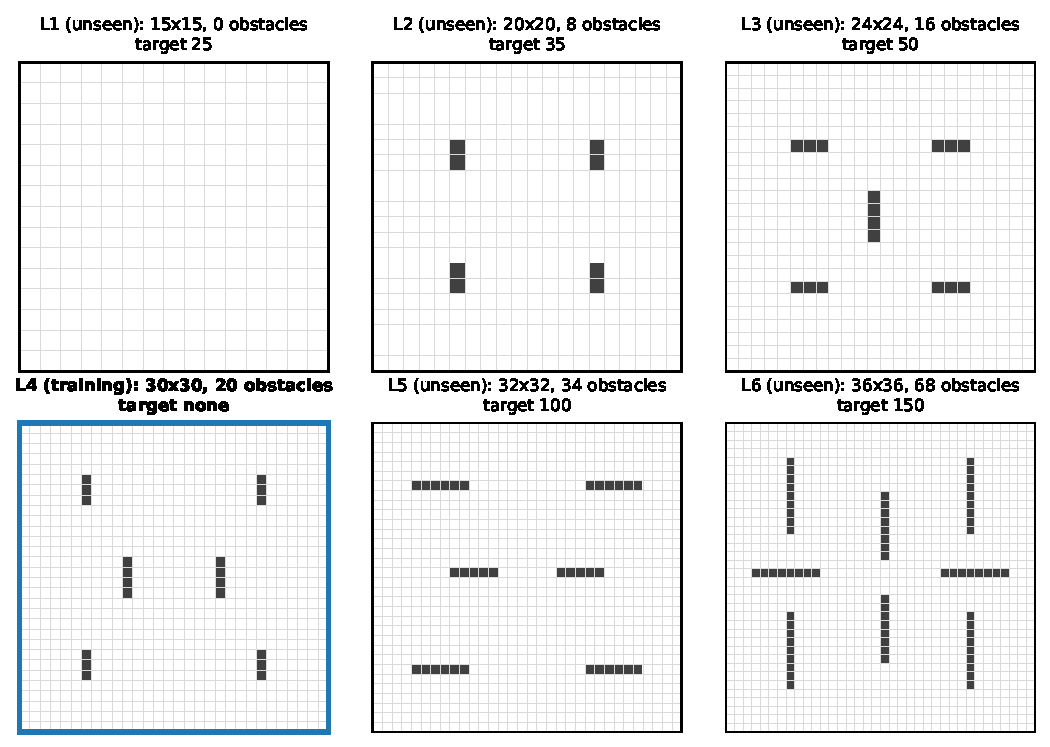
\includegraphics[width=0.82\textwidth]{generated/level_layouts.pdf}
  \caption{Obstacle layouts of the six levels, drawn from the configuration
  files. Each panel is scaled to the same display size; the grid shows the true
  board dimensions. Level~4 (outlined) is the only training environment.}
  \label{fig:level-layouts}
\end{figure*}

\Cref{fig:level-layouts} shows the layouts. Only Level~4 contributes
transitions to the replay buffer during the continuous training run. Consequently, Levels~1, 2, 3, 5, and 6 are all unseen by the
reported checkpoint, even though some configuration files retain metadata from
earlier versions of the project.

\subsection{Reward Function}

The reward at time $t$ is
\begin{equation}
  r_t =
  \begin{cases}
    +10, & \text{if food is consumed},\\
    -20, & \text{if a fatal collision occurs},\\
    -0.005 + 0.02, & \text{if the head moves closer to food},\\
    -0.005 - 0.02, & \text{otherwise},
  \end{cases}
  \label{eq:reward}
\end{equation}
where ``closer'' means that the move reduces the Manhattan distance between
the head and the food. The small distance-based shaping term encourages
progress toward food, while
the food and collision rewards remain the dominant signals. Rewards are used
only for learning. Evaluation reports the game score, i.e., the number of food
items eaten, so the shaping terms do not enter any reported metric.

\subsection{Action Space}

The agent selects one of three actions relative to its current heading:
\begin{equation}
  \mathcal{A}=\{\textsc{straight},\textsc{turn-right},\textsc{turn-left}\}.
\end{equation}
Relative actions avoid the ambiguity created by an absolute action that asks the
snake to reverse into its own body. They also preserve identical action
semantics across all board geometries.

\subsection{State Representation}

Every raw game state is encoded as a vector $s\in\mathbb{R}^{27}$. The feature
groups are listed in \cref{tab:state-features}.

\begin{table*}[t]
  \centering
  \caption{Fixed-dimensional state representation.}
  \label{tab:state-features}
  \begin{tabular}{clp{8.2cm}}
    \toprule
    Indices & Count & Description \\
    \midrule
    0--2   & 3 & Immediate danger for straight, right, and left actions \\
    3--6   & 4 & Current direction (up, down, left, right), one-hot encoded \\
    7--10  & 4 & Food location relative to the head \\
    11--13 & 3 & Normalized ray clearance for the three relative directions \\
    14--15 & 2 & Normalized row and column displacement to food \\
    16--17 & 2 & Normalized head position \\
    18     & 1 & Snake length divided by the number of usable cells \\
    19--21 & 3 & Reachable safe-area ratios after the three candidate actions \\
    22--25 & 4 & Tail location relative to the head \\
    26     & 1 & Normalized Manhattan distance from head to tail \\
    \bottomrule
  \end{tabular}
\end{table*}

Ray distances, coordinates, length, and head--tail distance are normalized by
the relevant board dimensions. Safe-area features use a bounded breadth-first
search after each candidate action to identify locally trapped states. The
fixed representation allows one network to process every level without padding
or resizing a raw grid.

\subsection{Dueling Double DQN}

The network has a shared multilayer perceptron with two 256-unit ReLU layers.
It then separates into a scalar value stream $V(s)$ and a three-output advantage
stream $A(s,a)$. They are combined as
\begin{equation}
  Q(s,a)=V(s)+A(s,a)-\frac{1}{|\mathcal{A}|}
  \sum_{a'\in\mathcal{A}}A(s,a').
  \label{eq:dueling}
\end{equation}

For transition $(s_t,a_t,r_t,s_{t+1},d_t)$, Double DQN first selects the next
action with the online network,
\begin{equation}
  a^*=\arg\max_a Q_{\theta}(s_{t+1},a),
\end{equation}
and evaluates it with the target network,
\begin{equation}
  y_t=r_t+\gamma(1-d_t)Q_{\bar{\theta}}(s_{t+1},a^*).
  \label{eq:double-target}
\end{equation}
The online parameters $\theta$ minimize the Huber loss between
$Q_{\theta}(s_t,a_t)$ and $y_t$. Gradients are clipped to a norm of 10, and the
target parameters $\bar{\theta}$ are periodically copied from the online
network.

\begin{table*}[t]
  \centering
  \caption{Hyperparameters of the continuous Level~4 training run.}
  \label{tab:hyperparameters}
  \begin{tabular}{lr@{\qquad}lr}
    \toprule
    Hyperparameter & Value & Hyperparameter & Value \\
    \midrule
    Learning rate & $3\times10^{-4}$ & Discount $\gamma$ & 0.995 \\
    Batch size & 256 & Replay capacity & 300,000 \\
    Replay warm-up & 5,000 & Target update period & 5,000 steps \\
    Training frequency & 2 steps & Hidden width & 256 \\
    Initial $\epsilon$ & 1.00 & Final $\epsilon$ & 0.01 \\
    Decay duration & 400,000 steps & Gradient norm limit & 10 \\
    Optimizer & Adam & Loss & Huber \\
    \bottomrule
  \end{tabular}
\end{table*}

\subsection{Single-Environment Training}

The agent was trained continuously on Level~4 using seed 0. Training was
interrupted during episode 19,095 after 14,293,725 environment steps; 19,094
completed episodes were recorded. At each 250-episode save point after a
500-episode warm-up, the trainer retained a candidate best checkpoint according
to the highest moving-average score over 100 training episodes. This criterion
selected the checkpoint at episode 17,000, where the moving average was 52.09.
The largest score observed in a completed training episode was 157.

These values characterize training only. They are not treated as independent
test performance because training episodes include the behavior policy and were
also used to select the checkpoint.

% =============================================================================
\section{Experimental Setup}
\label{sec:experimental-setup}

\subsection{Checkpoints and Baselines}

The primary model is
\path{results/level4_continuous_dqn/seed_0/checkpoint_best.pt}. The final
checkpoint at the end of training is evaluated as a sensitivity analysis. A
uniform random policy over the same three relative actions provides the minimum
baseline needed to distinguish learned transfer from chance behavior.

Training was performed on an NVIDIA RTX 5070 Ti. The independent evaluation was
executed on CPU at Git revision
\texttt{ec064486b98a12428bd4a4382e10166272d8d632}, using Python~3.12.13,
PyTorch~2.14.1, and NumPy~2.5.3. The full checkpoint SHA-256 hashes and the
environment-seed list are stored in
\path{results/cross_level_evaluation/metadata.json}. The evaluation command was
\path{python scripts/evaluate_cross_level.py --episodes 100}.

\subsection{Zero-Shot Evaluation Protocol}

Each checkpoint is frozen and evaluated with greedy action selection. No
transitions are stored, no gradients are computed, and no model parameter is
updated. Each model--level combination uses the same 100 episode seeds
(1234--1333). Evaluation is headless; rendering is reserved for qualitative
illustrations and is not used to compute results.

For every level, we report mean, standard deviation, median, quartiles, minimum,
and maximum score; episode length; steps per food; and rates of wall, obstacle,
self-collision, timeout, board-filled, and target-reached outcomes. For levels
with target score $T_l$, we additionally report
\begin{equation}
  \mathrm{SuccessRate}_l=\frac{1}{N}\sum_{i=1}^{N}
  \mathbb{I}\left[S_{i,l}\ge T_l\right]
  \label{eq:success}
\end{equation}
and normalized score
\begin{equation}
  \widetilde{S}_{i,l}=\min\left(\frac{S_{i,l}}{T_l},1\right).
  \label{eq:normalized-score}
\end{equation}
Level~4 has no target, so no post-hoc success threshold is introduced for that
level. Its in-domain performance is summarized by the full score and survival
distributions. Success rates are accompanied by two-sided 95\% Wilson score
intervals \cite{wilson1927probable}. These intervals quantify finite-sample uncertainty over evaluation
episodes and do not represent variability across independently trained agents.

Raw scores are not directly compared across all levels because board size,
target, and episode termination differ. We therefore avoid collapsing the study
into one generalization-gap value.

\subsection{Exploration Sensitivity}

A supplementary experiment re-evaluates the selected checkpoint with
$\epsilon=0.01$, the final exploration rate of the training behavior policy.
It uses the same 100 episode seeds on Levels~4, 5, and 6 and a separate,
fixed random-number generator for the exploratory actions. On Level~4, it tests
whether residual exploration explains the gap between training and evaluation
scores. On Levels~5 and 6, it tests whether occasional random actions change
the early timeouts reported in \cref{sec:results}. The results, configuration,
and checkpoint hash are stored in \path{results/epsilon_effect/} and were
produced by \path{python scripts/evaluate_epsilon_effect.py}.

\subsection{Reproducibility and Analysis}

All per-episode results were stored before aggregation, and the summary tables
and figures were generated automatically from those raw files. The evaluation
script recorded the model path, model hash, level configuration, random seed,
and code revision. Unless otherwise stated, variability in the evaluation
tables describes episodes under one trained policy and is not variation across
independently trained agents. In line with recommendations for empirical deep
RL, the analysis reports distributional summaries rather than relying on a
single mean score \cite{henderson2018deep,agarwal2021deep}.

% =============================================================================
\section{Results}
\label{sec:results}

\subsection{Training Behavior on Level 4}

\begin{figure}[t]
  \centering
  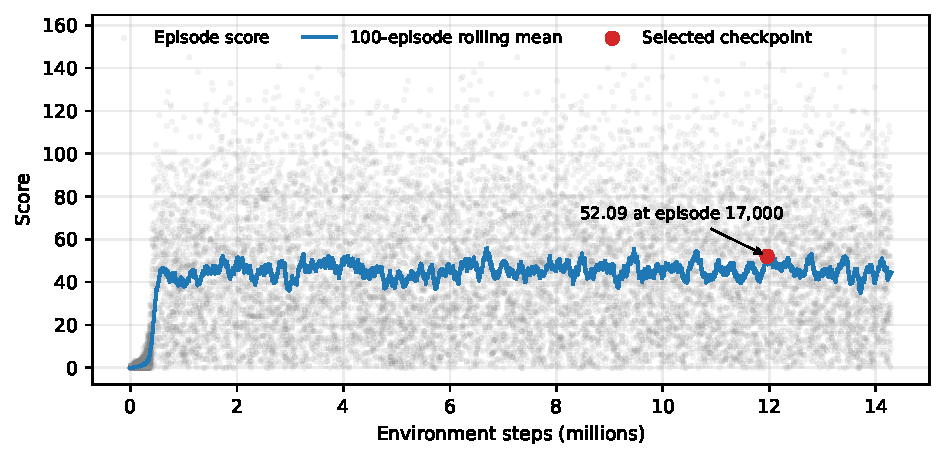
\includegraphics[width=\linewidth]{generated/training_curve.pdf}
  \caption{Training performance on Level~4. The moving average is descriptive
  of training and is not an independent evaluation result.}
  \label{fig:training-curve}
\end{figure}

Training ran for 14,293,725 environment steps and logged 19,094 completed
episodes (\cref{fig:training-curve}). Progress was initially slow: the mean
score was 0.03 over episodes 1--1,000 and 1.90 over episodes 5,001--6,000. The
rise coincided with the end of the exploration schedule. The exploration rate
$\epsilon$ reached its final value of 0.01 at episode 6,646 (400,901 steps),
and the mean score over episodes 7,001--8,000 was 43.5. After about 1.9 million
steps, the training score plateaued: every later block of 1,000 episodes had a
mean between 43.1 and 47.2. More than 85\% of the environment steps therefore
produced no further gain in this training metric.

The highest 100-episode moving average, 55.97, occurred at episode 12,326,
between two save points. Because the trainer compares candidates only at
250-episode save points, the selected checkpoint is the save-point maximum of
52.09 at episode 17,000. The moving average then declined to 46.04 by episode
19,000. The curve also shows substantial episode-level variation throughout.

\subsection{Cross-Level Performance}

\begin{table*}[t]
  \centering
  \caption{Greedy evaluation of the selected DQN checkpoint over 100 episodes
  per level. Success intervals are two-sided 95\% Wilson score intervals.}
  \label{tab:main-results}
  \begin{tabular}{lrrrrrrr}
    \toprule
    Level & Mean $\pm$ SD & Median & P25 & P75 & Success (\%) & 95\% CI & Norm. score \\
    \midrule
\tablerows{generated/main_results_rows.tex}
    \bottomrule
  \end{tabular}
\end{table*}

\Cref{tab:main-results} reports the primary zero-shot results. On the in-domain
Level~4, the selected checkpoint scored $144.49\pm27.28$ with a median of 154.
Without fine-tuning, it reached every Level~1 target and retained 97\% and 93\%
success on Levels~2 and 3. Transfer weakened on the larger layouts: success was
74\% on Level~5 and 54\% on Level~6. Their 95\% success intervals were
64.6--81.6\% and 44.3--63.4\%, respectively. The Level~6 interquartile range
extended from 1 to 150, revealing a strongly bimodal outcome in which the agent
often either reached the full target or made almost no progress.

\begin{figure}[t]
  \centering
  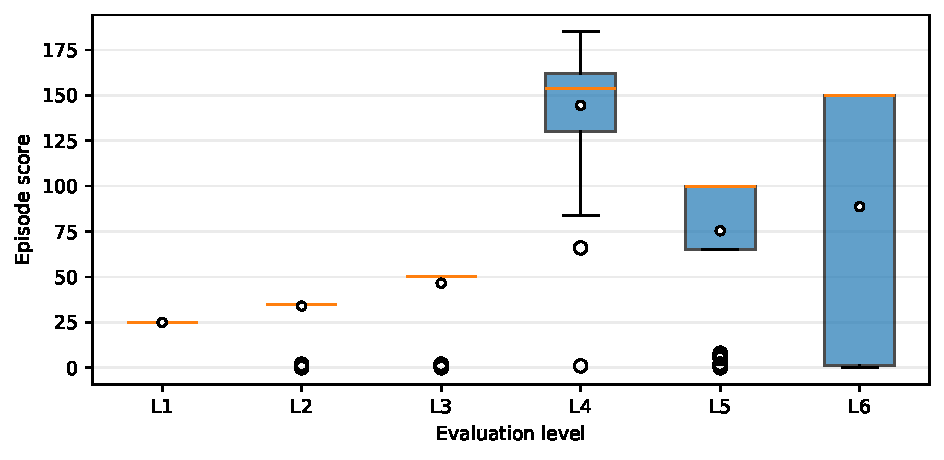
\includegraphics[width=\linewidth]{generated/score_distributions.pdf}
  \caption{Score distributions of the frozen DQN policy across six levels.}
  \label{fig:score-distributions}
\end{figure}

\subsection{Comparison with the Random Baseline}

\begin{table}[t]
  \centering
  \caption{Selected DQN versus a uniform random-action policy.}
  \label{tab:baseline}
  \begin{tabular}{lrrrr}
    \toprule
    & \multicolumn{2}{c}{Mean score} & \multicolumn{2}{c}{Success (\%)} \\
    \cmidrule(lr){2-3}\cmidrule(lr){4-5}
    Level & DQN & Random & DQN & Random \\
    \midrule
    1 & 25.00 & 0.10 & 100 & 0 \\
    2 & 33.98 & 0.08 & 97 & 0 \\
    3 & 46.58 & 0.03 & 93 & 0 \\
    4 & 144.49 & 0.03 & N/A & N/A \\
    5 & 75.40 & 0.02 & 74 & 0 \\
    6 & 88.71 & 0.02 & 54 & 0 \\
    \bottomrule
  \end{tabular}
\end{table}

The selected DQN exceeded the random baseline on every level. Random mean scores
ranged from 0.02 to 0.10 and it never reached a target, whereas the learned
policy's lowest target-level success rate was 54\%. The separation is also large
on the uncapped Level~4 (144.49 versus 0.03 mean score). This large descriptive
gap shows that the evaluated network learned behavior beyond merely executing
uniformly random valid relative actions.

\subsection{Best and Final Checkpoints}

The best and final checkpoints were evaluated under identical seeds. The final
checkpoint improved mean score on Level~4 from 144.49 to 153.83 and on Level~6
from 88.71 to 90.56. It also increased Level~2 success from 97\% to 99\%.
However, it reduced success from 93\% to 83\% on Level~3 and from 74\% to 65\%
on Level~5; Level~6 success changed from 54\% to 52\%.

\begin{table}[t]
  \centering
  \caption{Paired success comparison of the best and final checkpoints on the
  same 100 seeds per level. ``Best only'' counts seeds that only the best
  checkpoint solved. $p$ is the exact two-sided McNemar test; $p_\mathrm{Holm}$
  is adjusted over the five levels.}
  \label{tab:checkpoint-test}
  \begin{tabular}{lrrrrrr}
    \toprule
    Level & Best & Final & Best only & Final only & $p$ & $p_\mathrm{Holm}$ \\
    \midrule
\tablerows{generated/checkpoint_test_rows.tex}
    \bottomrule
  \end{tabular}
\end{table}

Because both checkpoints were evaluated on identical seeds, their success
outcomes form matched pairs. \Cref{tab:checkpoint-test} therefore applies an
exact two-sided McNemar test to the discordant seeds \cite{mcnemar1947note} and
controls the family-wise error over the five target levels with the Holm
procedure \cite{holm1979simple}. Only the Level~3 drop was nominally
significant ($p=0.041$; 15 seeds solved only by the best checkpoint versus 5
solved only by the final one), and no difference remained significant after
the Holm adjustment ($p_\mathrm{Holm}\ge0.207$). Later training improved the
in-domain score but did not consistently improve unseen-level transfer. With
100 seeds per level, the observed transfer differences between the two
checkpoints are not statistically reliable. For both checkpoints, the central
conclusion---substantial but incomplete cross-level generalization---is
unchanged.

\begin{figure}[t]
  \centering
  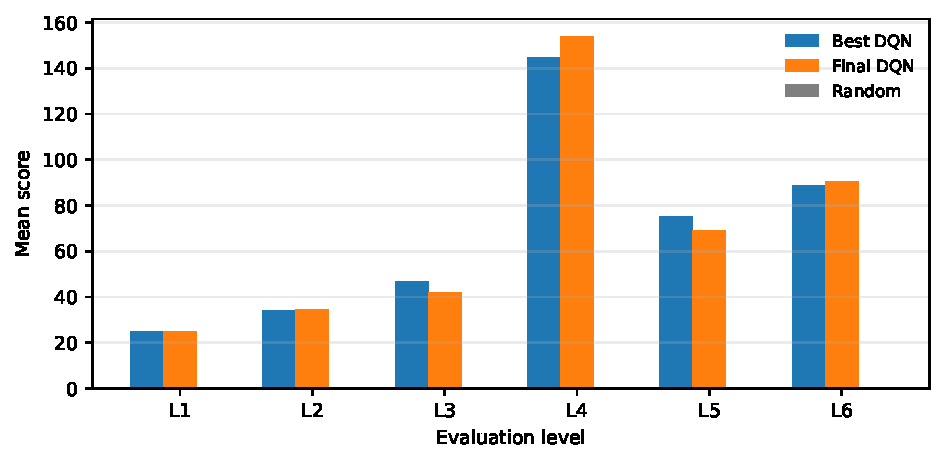
\includegraphics[width=\linewidth]{generated/checkpoint_comparison.pdf}
  \caption{Mean score of the selected checkpoint, final checkpoint, and random
  baseline under identical evaluation seeds.}
  \label{fig:checkpoint-comparison}
\end{figure}

\subsection{Termination and Failure Modes}

\begin{figure}[t]
  \centering
  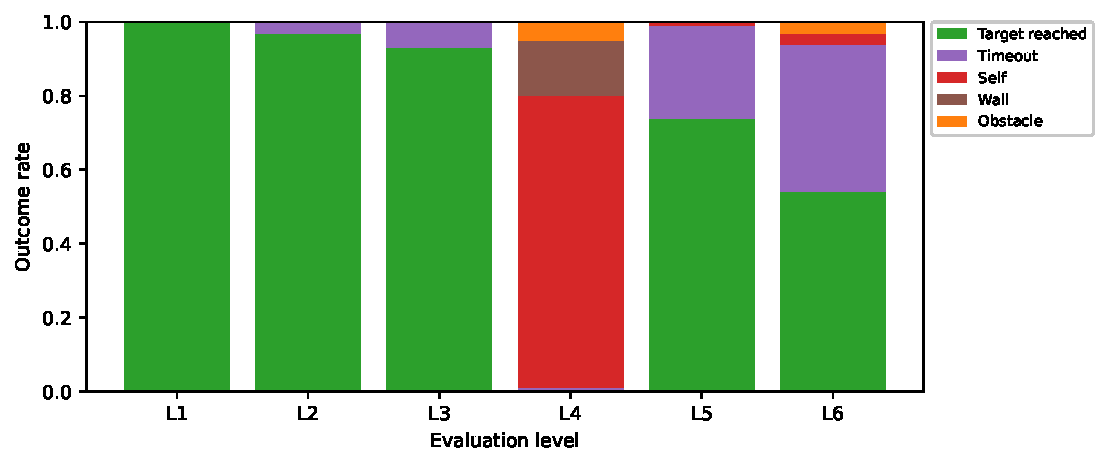
\includegraphics[width=\linewidth]{generated/failure_modes.pdf}
  \caption{Distribution of episode termination causes under greedy evaluation.}
  \label{fig:failure-modes}
\end{figure}

All Level~1 episodes reached the target. Failures on Levels~2 and 3 were solely
timeouts (3\% and 7\%, respectively). On uncapped Level~4, self-collision was
the dominant outcome (79\%), followed by wall collision (15\%), obstacle
collision (5\%), and timeout (1\%). Level~5 failures were mostly timeouts
(25\%), with 1\% self-collision. On Level~6, 40\% timed out, 3\% hit an
obstacle, and 3\% ended in self-collision. The learned policy had no wall
collisions outside Level~4.

\begin{table}[t]
  \centering
  \caption{Greedy failures of the selected checkpoint on the levels with a
  target. Median, max, and the last column refer to the score at the moment of
  timeout.}
  \label{tab:timeouts}
  \begin{tabular}{lrrrrr}
    \toprule
    Level & Failures & Timeouts & Median & Max & Score $\le2$ \\
    \midrule
\tablerows{generated/timeout_rows.tex}
    \bottomrule
  \end{tabular}
\end{table}

\Cref{tab:timeouts} shows when these timeouts occurred. Every timeout on
Levels~2, 3, 5, and 6 happened at a score of at most 9, and the median score at
timeout was 1 on every level. On Level~6, 34 of the 40 timeouts occurred after
two or fewer food items. The dominant failure on unseen levels is therefore an
early stall of a short snake, not a late collapse of a long one. Conversely,
episodes that reached a score of 10 almost always finished: 318 of 325 such
episodes on Levels~2, 3, 5, and 6 reached the target. The seven exceptions were
late collisions at scores between 84 and 146.

\subsection{Sensitivity to Residual Exploration}

\begin{table}[t]
  \centering
  \caption{Selected checkpoint under greedy control ($\epsilon=0$) and with
  $\epsilon=0.01$ on the same 100 seeds. Success, timeout, and collision
  (wall, obstacle, or self) are percentages of episodes.}
  \label{tab:epsilon}
  \setlength{\tabcolsep}{3.5pt}
  \begin{tabular}{lrrrrrr}
    \toprule
    Level & $\epsilon$ & Mean $\pm$ SD & Median & Success & Timeout & Collision \\
    \midrule
\tablerows{generated/epsilon_rows.tex}
    \bottomrule
  \end{tabular}
\end{table}

The greedy rows of \cref{tab:epsilon} reproduce \cref{tab:main-results}
exactly. With $\epsilon=0.01$, the Level~4 mean fell from 144.49 to 43.58
(median 41), close to the 1,000-episode training means of 43.1--47.2 reported
above. On Levels~5 and 6, the same small amount of randomness nearly eliminated
timeouts, from 25\% to 0\% and from 40\% to 1\%. However, collisions rose to
96\% and 99\% of episodes, and success fell from 74\% to 4\% and from 54\% to
0\%.

% =============================================================================
\section{Discussion}
\label{sec:discussion}

\subsection{RQ1: In-Domain Performance}

The selected checkpoint performed strongly on its training environment under
independent greedy evaluation, with a mean score of 144.49, a median of 154,
and a standard deviation of 27.28. The interquartile range was 130.25--162.25,
although the minimum of 1 shows that occasional catastrophic episodes remained.
The final checkpoint raised the mean to 153.83 but also had a larger standard
deviation of 31.53. These evaluation scores are about three times the training
moving average. The exploration experiment in \cref{tab:epsilon} explains the
gap: adding the behavior policy's final $\epsilon=0.01$ back to the frozen
network lowers its Level~4 mean to the level observed during training. A single
random action is often fatal for a long snake on a board with obstacles. The
training curve therefore understates the greedy policy and should not be read
as its test performance.

\subsection{RQ2: Zero-Shot Cross-Level Transfer}

The frozen policy demonstrated transfer beyond technical executability. It
reached the target in 100\% of Level~1 episodes, 97\% of Level~2 episodes, and
93\% of Level~3 episodes. It also transferred to boards larger than the source
environment, succeeding in 74\% of Level~5 episodes and 54\% of Level~6
episodes. In contrast, the random policy reached no target and averaged at most
0.10 food per episode. We therefore find strong transfer to the three smaller
levels and meaningful but unreliable transfer to the two larger challenge
levels. For this training run, the result supports cross-level generalization
within the evaluated suite, but not uniformly robust behavior across all
layouts.

Transfer to smaller boards and transfer to larger, obstacle-dense boards need
not have the same difficulty. A smaller board reduces travel distance but also
reduces maneuvering space, whereas a larger board increases both search distance
and the number of configurations encountered before the snake becomes long.
The final interpretation must be based on the observed score and failure-mode
distributions rather than board size alone.

\subsection{RQ3: Effects of Environment Geometry}

Performance generally became less reliable as the test environments grew and
their targets increased. The failure analysis in \cref{tab:timeouts} locates
this weakness precisely. On every unseen level with a target, failures were
dominated by no-food timeouts, and those timeouts occurred almost exclusively
at the start of an episode, with a median score of 1. Once the snake had eaten
ten items, the policy reached the target in 318 of 325 episodes. The 1--150
interquartile range on Level~6 is a direct consequence: an episode either
stalls almost immediately or runs to completion. The limiting factor for
transfer is therefore not collision avoidance with a long body but the
policy's behavior while the snake is still short.

The exploration experiment adds evidence about these stalls. Between two food
items, both the greedy policy and the environment are deterministic, so a
no-food timeout means that the snake moved for twice the number of board cells
without reaching the food. With $\epsilon=0.01$, such timeouts nearly vanished on Levels~5 and
6. The stalls are therefore not robust to small perturbations, which is
consistent with non-progressing cycles of the greedy policy. Because the
experiment records only episode outcomes, it cannot separate episodes that
escaped a cycle from episodes that a random action ended before the timeout.
The collapse in success shows, however, that uniform random perturbation is not
a remedy: the randomness that breaks a stall is often fatal later in the
episode. A targeted mechanism, such as perturbing actions only after a repeated
state is detected, is a natural next step but was not evaluated here.

Level~4 presents a different failure profile: 79\% of episodes eventually
ended in self-collision. This is not evidence of weaker short-horizon control;
because Level~4 has no score target, successful trajectories continue until the
long snake ultimately collides or times out. The higher collision rate is
therefore partly a consequence of its uncapped termination rule. More broadly,
the observed differences cannot be assigned uniquely to board size or obstacle
layout because target, size, and geometry change together.

The 27-feature representation and relative actions are plausible mechanisms for
transfer because their dimensionality and semantics do not change between
levels. Nevertheless, the present design does not isolate their causal effect.
An ablation study would be required to attribute performance gains to individual
feature groups, relative actions, or reward shaping.

\subsection{Threats to Validity}

The study has several limitations. First, the reported model comes from one
training seed, so the evaluation quantifies stochastic environment outcomes for
one learned policy rather than variation across independent training runs.
Second, training uses only one source level; the findings may depend strongly on
the choice of Level~4. Third, evaluation levels change several factors
simultaneously, including board size, obstacle count, obstacle geometry, and
target score. Their individual effects therefore cannot be identified.

Fourth, the best checkpoint is selected using a moving average of training
episodes, not a separate validation environment. Fifth, raw scores are not
fully comparable because Level~4 is uncapped while other levels terminate at a
target. Sixth, no ablation isolates the contributions of state features, reward
shaping, or relative actions. Finally, a finite collection of five unseen
levels supports conclusions only about this test suite, not arbitrary Snake
environments.

% =============================================================================
\section{Conclusion}
\label{sec:conclusion}

This work examines cross-level generalization of a Dueling Double DQN trained
on a single parameterized Snake environment. The agent uses a fixed 27-feature
state representation and three relative actions, allowing one frozen network to
run on boards with different sizes and obstacle layouts. The evaluation compares
the training level with five unseen levels and includes a random-policy baseline.

For the evaluated training run, the selected checkpoint achieved an in-domain
Level~4 score of
$144.49\pm27.28$ and transferred without fine-tuning with success rates of
100\%, 97\%, 93\%, 74\%, and 54\% on Levels~1, 2, 3, 5, and 6. It exceeded the
random baseline on every level, but high variance and timeout rates on Levels~5
and 6 indicate that generalization weakened as the evaluation environments
became larger and more demanding. Later training improved the Level~4 mean to
153.83 but reduced success on Levels~3 and 5. Those reductions were not
significant after correction for multiple comparisons, so stronger in-domain
performance did not translate into reliably stronger transfer.

Failure analysis located the main weakness at the start of an episode: on
unseen levels, most failures were no-food timeouts at a median score of 1,
while episodes that passed ten food items almost always reached the target.
Uniform random perturbation removed these timeouts but caused far more
collisions.

Future work should repeat training over multiple seeds, introduce additional
held-out layouts, isolate representation and reward components through ablation,
test targeted mechanisms that break non-progressing cycles, and compare
single-level training with domain randomization or curriculum learning under an
equal environment-step budget.

% =============================================================================
% Bibliography. Build order: pdflatex -> bibtex -> pdflatex -> pdflatex.
% =============================================================================
\bibliographystyle{IEEEtran}
\bibliography{references}

\end{document}
